\chapter{Конструкторский раздел}

В данном разделе будут спроектированы схемы алгоритмов, описаны используемые типы данных, а также произведена оценка памяти и описана структура ПО.

\section{Схемы алгоритмов}

На рисунках 2.1 - 2.2 представлены схемы рассматриваемых алгоритмов.

На рисунках 2.3 - 2.5 представлены схемы используемых в муравьином алгоритме функций.

\begin{figure}[H]
	\begin{center}
		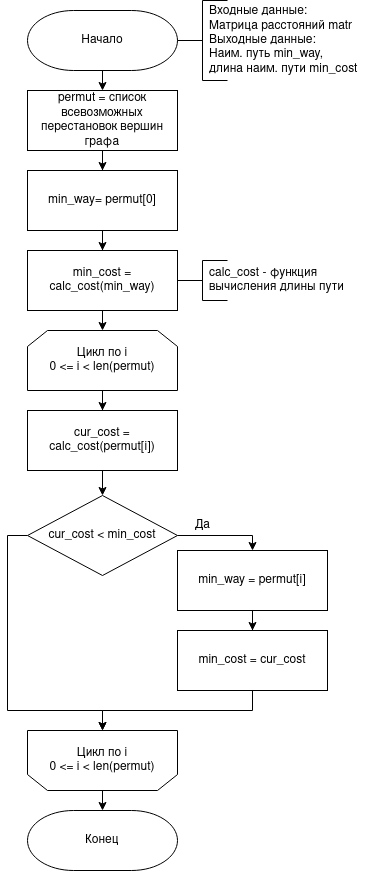
\includegraphics[scale=0.6]{assets/enum.png}
	\end{center}
	\caption{Схема алгоритма полного перебора}
\end{figure}

\begin{figure}[H]
	\begin{center}
		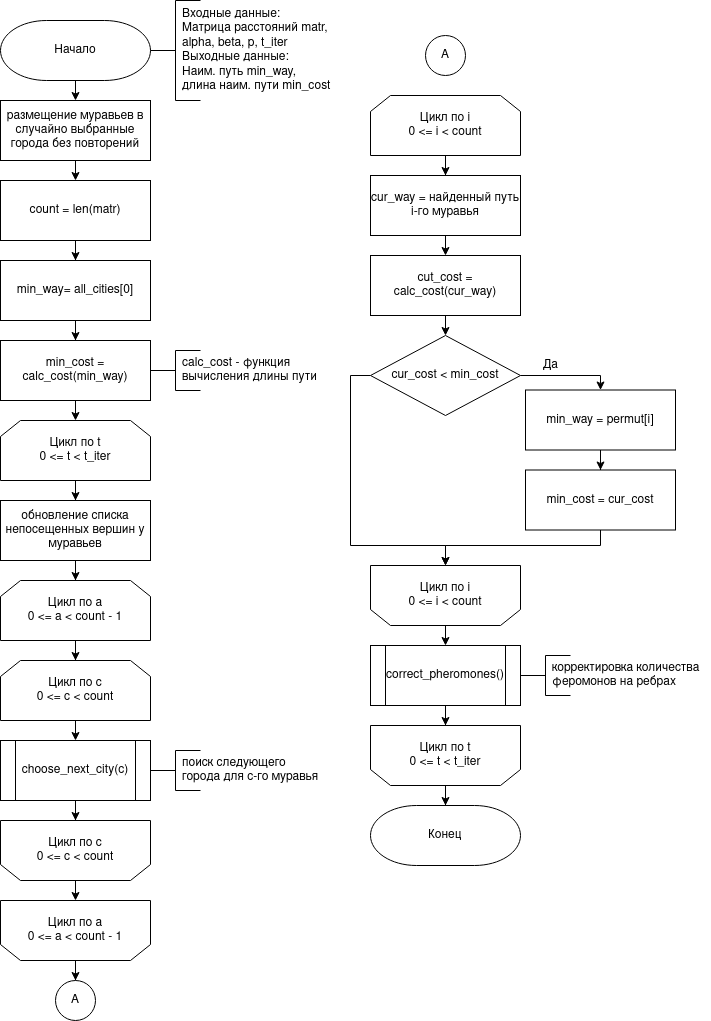
\includegraphics[scale=0.6]{assets/antMain.png}
	\end{center}
	\caption{Схема муравьиного алгоритма}
\end{figure}

\begin{figure}[H]
	\begin{center}
		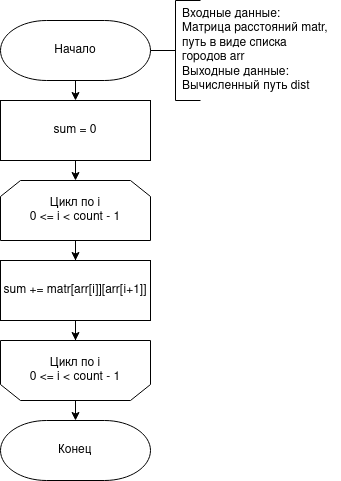
\includegraphics[scale=0.6]{assets/calc_dist.png}
	\end{center}
	\caption{Функция вычисления расстояния пути}
\end{figure}

\begin{figure}[H]
	\begin{center}
		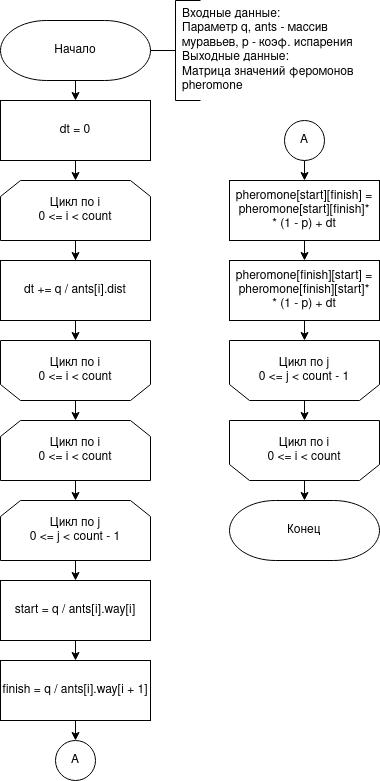
\includegraphics[scale=0.6]{assets/cor_pher.png}
	\end{center}
	\caption{Функция корректировки феромонов}
\end{figure}

\begin{figure}[H]
	\begin{center}
		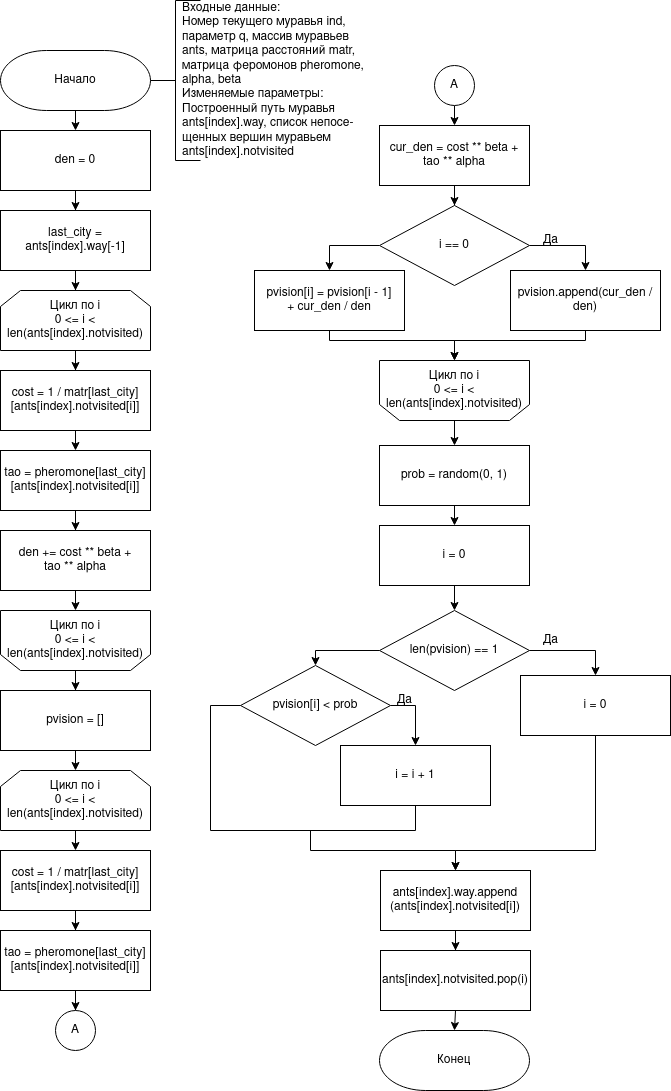
\includegraphics[scale=0.6]{assets/next_city.png}
	\end{center}
	\caption{Функция выбора муравьем следующего города}
\end{figure}

\newpage
\section{Используемые типы данных}

\captionsetup{singlelinecheck = false, justification=raggedright}
При реализации алгоритмов будут использованы следующие структуры данных:
\begin{itemize}
	\item муравьиная колония AntColony;
	\begin{lstlisting}[caption= Класс AntColony]
	class AntColony(object):
		def __init__(self, distances, decay, tmax, alpha=0.5,\
		 beta=0.5, e=0):
			self.distances = distances
			for i in range(len(distances)):
				for j in range(len(distances)):
					if self.distances[i][j] == 0:
						self.distances[i][j] = 10000000
			self.pheromone = np.ones(self.distances.shape)\
			 / len(distances)
			self.all_inds = list(range(len(distances)))
			self.decay = decay
			self.alpha = alpha
			self.beta = beta
			self.tmax = tmax
			self.count = len(distances)
			self.ants = []
			self.n_elits = e
			self.q = sum([sum(x) for x in distances])*2
	\end{lstlisting}
	Она имеет следующие поля:
	\begin{enumerate}
		\item distances - матрица расстояний;
		\item pheromone - матрица значений феромонов;
		\item all\_inds - упорядоченный список всех вершин графа;
		\item decay - коэффициент испарения;
		\item alpha - коэффициент $\alpha$;
		\item beta - коэффициент $\beta$;
		\item tmax - количество итераций;
		\item count - количество вершин в графе;
		\item ants - список объектов муравьёв;
		\item n\_elits - количество "элитных" муравьёв;
		\item q - коэффициент q.
	\end{enumerate}
	\item муравей Ant.
	\begin{lstlisting}[caption = Класс Ant]
	class Ant(object):
		def __init__(self):
			self.way = []
			self.start = 0
			self.dist = 0
			self.notvisited = []
	\end{lstlisting}
	Она имеет следующие поля:
	\begin{enumerate}
		\item way - текущий путь муравья;
		\item start - вершина, с которой муравей начинает свой путь;
		\item dist - длина найденного кратчайшего пути;
		\item notvisited - список непосещенных вершин.
	\end{enumerate}
\end{itemize}
\captionsetup{singlelinecheck = false, justification=centering}

\section{Оценка памяти}

Рассмотрим затрачиваемый объем памяти для рассмотренных алгоритмов. 

При полном переборе память используется на:
\begin{itemize}
	\item размер матрицы расстояний n - sizeof(int);
	\item матрица расстояний - n * n * sizeof(int);
	\item вспомогательные переменные - 4 * sizeof(int);
	\item вспомогательный список всевозможных перестановок вершин графа - n! * sizeof(int).
\end{itemize}

При использовании муравьиного алгоритма помимо матрицы расстояний и ее размера используются также:
\begin{itemize}
	\item размер полей класса AntColony - sizeof(AntColony);
	\item муравьи класса Ant - k * sizeof(Ant);
	\item вспомогательные переменные - ~15 * sizeof(double).
\end{itemize}

Таким образом, муравьиный алгоритм значительно увеличивает количество используемой памяти из-за используемых структур и классов, а также большего числа вспомогательных переменных.

\section{Структура ПО}

ПО будет состоять из следующих модулей:
\begin{itemize}
	\item главный модуль - из него будет осуществляться запуск программы и выбор соответствующего режима работы;
	\item модуль интерфейса - в нем будет описана реализация режимов работы программы;
	\item модуль, содержащий реализации алгоритмов.
\end{itemize}

\section{Вывод}

На основе полученных в аналитическом разделе знаний об алгоритмах были спроектированы схемы алгоритмов, выбраны используемые типы данных, проведена оценка затрачиваемого объема памяти, а также описана структура ПО.